\paragraph{}
Графы являются одной из основных структур в информатике, а алгоритмы над ними чрезвычайно важны в анализе компьютерных и социальных сетей, статическом анализе кода, биоинформатике~\cite{gb_math}. Графы, возникающие в данных областях, могут содержать миллионы узлов и ребер, поэтому распараллеливание алгоритмов для работы с ними оказывается необходимым условием достижения высокой производительности. Однако такое улучшение их эффективности происходит за счет более сложной модели программирования~\cite{blast}. Результатом этого становится, в том числе, несоответствие между языками высокого уровня, на которых пользователи и разработчики графовых алгоритмов предпочли бы программировать (например, Python), и языками программирования для параллельного оборудования~\cite{blast}. Таким образом, существующие решения либо просты в использовании (networkx\footnote{Репозиторий библиотеки networkx: \url{https://github.com/networkx/networkx}. Дата посещения: 13.12.2020}), либо высокопроизводительны (gunrock\footnote{Репозиторий библиотеки gunrock: \url{https://github.com/gunrock/gunrock} Дата посещения: 13.12.2020}). Проблемой является и то, что традиционные параллельные алгоритмы для анализа графов тяжело реализовывать и оптимизировать, а прирост производительности от роста числа параллельных процессов снижается~\cite{gb_math}. 

С появлением эффективных структур и алгоритмов для разреженных матриц становится возможным использование подхода к вычислению над графами, основанного на линейной алгебре. Матрица смежности может представлять широкий спектр графов, включая ориентированные, взвешенные, двудольные. Ключевым свойством такого подхода является способность оперировать богатым набором графов различных типов с помощью небольшого набора матричных операций над полукольцами. Например, транспонирование матрицы смежности изменяет направления ребер в ориентированном графе, а умножение матрицы на вектор, как показано на рисунке~\ref{fig:bfs_step}, является шагом в алгоритме поиска в ширину.

\begin{figure}[h!]
    \centering
    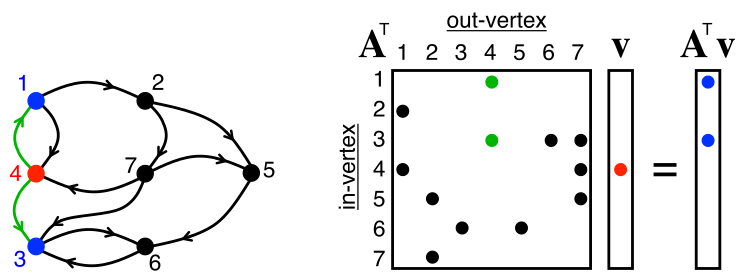
\includegraphics[width=0.9\linewidth]{pictures/MatrixBFS.png}
    \caption{Вычисление одного шага в алгоритме поиска в ширину\footnotemark}
    \label{fig:bfs_step}
\end{figure}

Спецификация GraphBLAS~\cite{gb_math} определяет базовые примитивы для построения графовых алгоритмов в терминах линейной алгебры. Разработчики считают, что эта область достаточно зрела, чтобы иметь потребность в стандартизации. Стандартизация позволяет сконцентрировать усилия исследователей на разработке инновационных алгоритмов для анализа и обработки графов, а не придумывать все новые, во многом пересекающиеся, низкоуровневые решения. Кроме того, благодаря такому подходу, по словам авторов\cite{sevengr}, возможно решение некоторых проблем, описанных ниже.
\begin{enumerate}
    \item \textbf{Переносимость.} Алгоритмы не требуют модификаций для достижения высокой производительности на конкретном устройстве.
    \item \textbf{Лаконичность.} Алгоритмы выражаются гораздо меньшим числом строчек кода.
    \item \textbf{Производительность.} Алгоритмы остаются высокопроизводительными.
    \item \textbf{Масштабируемость.} Алгоритмы эффективны как на небольших, так и на огромных данных.
\end{enumerate}

\footnotetext{GraphBLAS [Электронный ресурс] // Википедия. Свободная энциклопедия. – URL: \url{https://en.wikipedia.org/wiki/GraphBLAS} (дата обращения: 13.12.2020).}

GraphBLAS описывает небольшое множество математических операций, которые необходимы для реализации широкого спектра операций над графами. В стандарте описаны следующие объекты:
\begin{itemize}
    \item абстрактные структуры для хранения дынных (матрицы, векторы)
    \item алгебраические структуры (моноиды, полукольца, бинарные и унарные операторы)
    \item операции линейной алгебры над произвольными алгебраическими структурами (произведение матриц, поэлементное сложение и умножение, взятие подматрицы и т.д.)
    \item объекты управления (маски и дескрипторы)
\end{itemize}

На данный момент стандарт GraphBLAS уже имеет несколько полноценных реализаций\footnote{Форум, посвященный стандарту GraphBLAS: \url{https://graphblas.github.io/}. Дата посещения: 04.06.2021}, однако все они в основном ориентированы на исполнение на CPU. В то же время разработка инструмента с поддержкой исполнения на графических процессорах общего назначения является перспективным направлением исследований, так как их использование может существенно повысить производительность такого рода решений\cite{gbtl}\cite{blast}. На текущий момент нет стандартного подхода к реализации спецификации GraphBLAS на GPU --- разработчики сталкиваются не только с проблемами, связанными с реализацией обобщенных операций на графических процессорах с помощью стандартных инструментов языка C++, но и с переносимостью решений, основанных на программно-аппаратной платформе CUDA. Одним из возможных подходов к реализации GraphBLAS на GPU является использование языка высокого уровня, а также библиотек, динамически транслирующих конструкции и объекты данного языка в низкоуровневый код, способный исполнятся на графическом процессоре видеокарты. 
